\documentclass{chi2009}
\usepackage{times}
\usepackage{url}
\usepackage{graphics}
\usepackage{color}
\usepackage[pdftex]{hyperref}
\hypersetup{%
pdftitle={TwinList: \\ Visualizing List Differences},
pdfauthor={Leonardo Max Baptista Claudino, claudino@cs.umd.edu \\
	    Sameh Khamis, sameh@cs.umd.edu \\
	    Ran Liu, ranliu@cs.umd.edu \\
	    Ben London, blondon@cs.umd.edu \\
	    Jay Pujara, jay@cs.umd.edu},
pdfkeywords={list visualization},
bookmarksnumbered,
pdfstartview={FitH},
colorlinks,
citecolor=black,
filecolor=black,
linkcolor=black,
urlcolor=black,
breaklinks=true,
}
\newcommand{\comment}[1]{}
\definecolor{Orange}{rgb}{1,0.5,0}
\newcommand{\todo}[1]{\textsf{\textbf{\textcolor{Orange}{[[#1]]}}}}

% TwinList Macros
\newcommand{\TwinList}{\textsc{TwinList}}
\newcommand{\ListViewer}{\textit{List Viewer}}
\newcommand{\AcceptReject}{\textit{Accept/Reject}}
\newcommand{\AcceptedRejected}{\textit{Accepted/Rejected}}
\newcommand{\Controls}{\textit{Control Panel}}
\newcommand{\Filters}{\textit{Filter Panel}}
\newcommand{\Details}{\textit{Details Panel}}
\newcommand{\GroupBy}{\textit{Group By}}
\newcommand{\SortBy}{\textit{Sort By}}
\newcommand{\Similar}{\textit{Similar}}
\newcommand{\Identical}{\textit{Identical}}

\pagenumbering{arabic}  % Arabic page numbers for submission.  Remove this line to eliminate page numbers for the camera ready copy

\begin{document}
% to make various LaTeX processors do the right thing with page size
\special{papersize=8.5in,11in}
\setlength{\paperheight}{11in}
\setlength{\paperwidth}{8.5in}
\setlength{\pdfpageheight}{\paperheight}
\setlength{\pdfpagewidth}{\paperwidth}

% use this command to override the default ACM copyright statement 
% (e.g. for preprints). Remove for camera ready copy.
\toappear{Submitted for CMSC 734 Information Visualization.}

\title{TwinList: \\ Visualizing List Differences}
\numberofauthors{5}
\author{
  \alignauthor Leonardo Claudino \\
    \affaddr{Dept. of Computer Science, University of Maryland}\\
    \affaddr{College Park, MD 20742}\\
    \email{claudino@cs.umd.edu}
  \and
  \alignauthor Sameh Khamis\\
    \affaddr{Dept. of Computer Science, University of Maryland}\\
    \affaddr{College Park, MD 20742}\\
    \email{sameh@cs.umd.edu}
  \and
  \alignauthor Ran Liu \\
    \affaddr{Dept. of Computer Science, University of Maryland}\\
    \affaddr{College Park, MD 20742}\\
    \email{ranliu@cs.umd.edu}
  \and
  \alignauthor Ben London \\
    \affaddr{Dept. of Computer Science, University of Maryland}\\
    \affaddr{College Park, MD 20742}\\
    \email{blondon@cs.umd.edu}
  \and
  \alignauthor Jay Pujara \\
    \affaddr{Dept. of Computer Science, University of Maryland}\\
    \affaddr{College Park, MD 20742}\\
    \email{jay@cs.umd.edu}
}

\maketitle

\begin{abstract}
We present a novel list visualization tool named $\TwinList$, for the purpose of list visualization and matching. Leveraging Adobe's Flex platform and the Prefuse Flare toolbox, we created a rich internet application (RIA) with dynamic animated effects. These animated transitions lead the user through the procedure of matching two lists, using color coding to highlight the similarities and differences between the two. List items can be grouped, sorted and filtered according to their attribute values, to enhance workflow. To illustrate the efficacy of the application, we conduct usability testing for different applications with several domain experts and peers.
\end{abstract}

\keywords{list visualization} 

\category{H.5.2}{Information Interfaces and Presentation}{Miscellaneous}

\section{Introduction}
A common task is comparing information from different sources or about different entitites. This problem occurs in everyday life as well as in specialized applications. For example, a consumer interested in making a purchase may wish to compare the features of two products. A newspaper may wish to compare the words used by different political parties during campaign speeches. Or as a more specialized example, a doctor performs the task of medical reconciliation. In medical reconciliation, a doctor crafting a treatment plan for a patient prior to their discharge from a hospital will need to compare medications the patient was taking before admission with the medications administered during hospitalization. 

A core problem shared by these applications is that data is in the form of two lists, and a decision is reached by comparing the constitutent items of these lists in a structured way. One element of the list structure is that items have some similiarity or correspondence between lists. The logic necessary to compare these items can be complicated, such as resolving a prescription drug and its generic equivalent as the same item in two different lists. Each item may have attributes that must be taken into consideration when assessing simililarity, such as the dosage of a medication prescribed. Attributes may also be used to segment list items into categories, such as different classes of drugs. Finally, list comparison should help reach a conclusion, such as a purchasing decision or a final list of medications to prescribe a patient.

Our goal was to design a visualization that allows users to quickly answer the dual questions ``What is the same between these two lists?'' and ``What is different between these two lists?'', quickly, accurately and effortlessly. We address these aspects of the list comparison problem in our visualization tool, $\TwinList$. Using a spatial organization of data, we provide an intuitive way for users to quickly differentiate between items that are the same and those that differ in two lists of data. We abstract complicated similarity logic by categorizing items as ``identical'' when they are the same in both lists, ``unique'' when they appear in only one lists, and ``similar'' when the same item has different attributes in each list. We map these three categories to a workflow and use animation to help users understand each step of the list comparison process. In addition, $\TwinList$ provides sorting, filtering, and grouping functionality to allow users to explore different aspects of the data. Finally, the application supports choosing items that are relevant or irrelevant, helping users reach a strong conclusion. 


\subsection{Related Work}
\todo{Does anyone want to take a crack at this?}

\section{TwinList}
$\TwinList$ is a novel list visualization tool for the purpose of illustrating the similarities and differences between two lists. It can be used in many cases where the comparison of two lists of items is required. The primary application that $\TwinList$ supports is that of medication list reconciliation: comparing and reconciling multiple medications that have been prescribed to a patient from multiple sources\cite{JCAHO-2006}. However, $\TwinList$ is equally adept in other applications, such as comparing bag-of-words lists or visualizing gene activity in different types of human tissue, such as normal brain tissue and brain tumor tissue.

$\TwinList$ interface consists of four major components: the $\ListViewer$, $\Controls$, $\AcceptedRejected$ lists and $\Details$, as shown in (Figure~\ref{fig:interface}). $\ListViewer$ is located in the upper left corner of the interface.This is where the list matching visualization will be performed. The initial view is two separated lists loaded from a input XML file.  $\Controls$ at the upper right corner, the controls, options and filters of the visualization can be found in this panel. If an item is selected, its detail information will be shown in the detail panel at the lower right corner. TwinList allows users to take actions to the list items, such as accept or reject list items. The results of the action will be displayed in the $\AcceptedRejected$ list. 


\begin{figure}
\begin{center}
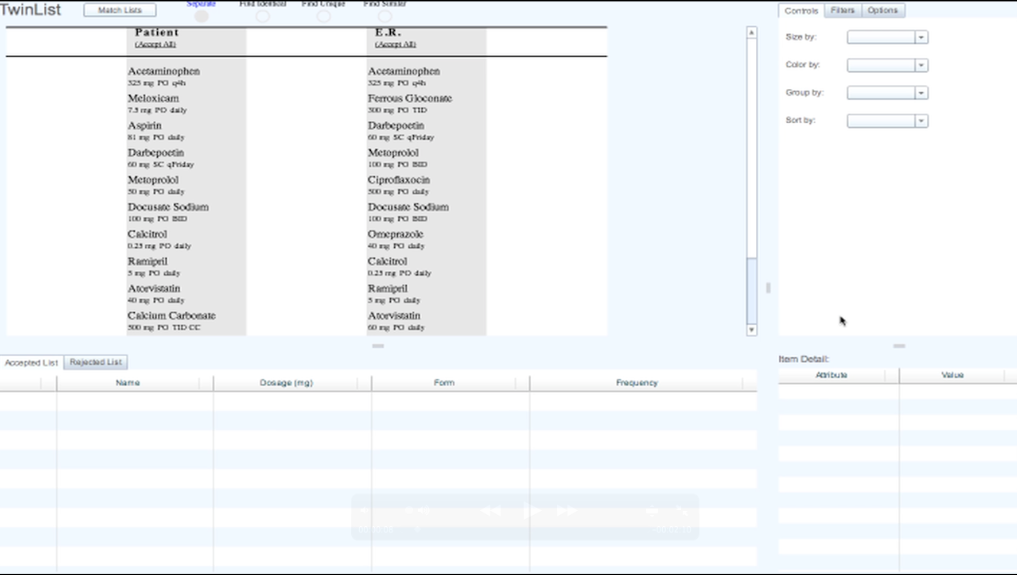
\includegraphics[width=1.1\linewidth]{interface}
\end{center}
   \caption{$\TwinList$ interface}
   \label{fig:interface}
\end{figure}

\subsection{ListViewer}
 \todo{I think we should find out a way to cite the Shneiderman's "golden rules" somewhere and state how our visualization design satisfy the rules}
\subsubsection{The five-column list placement}
\subsubsection{Matching Animation}

\subsection{Controls}

\subsection{Filters}

\subsection{Options}

\section{Evaluation}
Our goal was to deliver a working prototype, not a finished, fully-functional application. As such, we are more concerned with qualitative than quantitative feedback on the features of our visualization system at this point. According to the categorization proposed by Lam et al~\cite{lam-bertini-isenberg-plaisant-carpendale-2011}, the evaluation scenario best matching our present purposes is the \textit{User Experience (UE)} test case. The goal of the following experiments is to observe how users react to the visualization and interaction features offered by $\TwinList$. We will use their feedback to improve the system's design in future versions.

\subsection{Experiment Design}
Our test subjects came from two populations: two physicians and two non-specialist participants. The former used $\TwinList$ to perform medication reconciliation; the latter to fine interesting insights in bag-of-words data from two State of Union speeches. The testing protocol proceeded as follows: first, the user watched a $~7$-minute video demonstrating basic usage. Following this, the user was allowed to ask questions. Next, the user interacted with the system unaided, performing either specific tasks (medication reconciliation case studies) or exploratory analysis (State of the Union comparison). While using the system, subjects were encouraged to \textit{think aloud}~\cite{lewis-1982}. The entire experiment was captured in both audio and screen capture video.

\subsection{Case 1: Med. reconciliation, A. Z. H., male, 34 y. o.}
Overall, the participant performed the tasks as expected and reported anticipated results. A. Z. H. purported to be very comfortable with computers. He does not perform medication reconciliation on a regular basis, except when doing inpatient aid and discharge from the hospital, for which he does not use any software. This is how he describes his $\TwinList$ experience: \textit{``It's really impressive, the way you organize things is great. It's definitely a step in the right direction \dots"}. He was very enthusiastic and provided several suggestions, most of all worth including in this section. 

\subsubsection{Results}
This is our reading of A. Z. H.'s experience:
\begin{itemize}
\item There is need for an indication that there are more items than what can be currently seen in a column. The scroll bar alone is insufficient.
\item It is difficult to get to the $\AcceptReject$ pop-up menu when accepting/rejecting an item. He had trouble with the click-and-hold behavior, wanting instead to use the mouse's right-click button.
\item To send items from $\AcceptedRejected$ lists back to the viewer one-by-one requires quite some effort when you have many items in those lists. A \textit{Remove All} button would be desirable.
\item Warning dialogs or undo may be needed when accepting and rejecting items, since it is a delicate operation in medication reconciliation.
\item In the control panel, drop-down boxes should indicate what the default $\GroupBy$/$\SortBy$ attributes are, instead of blank captions. (The default is actually the original ordering.)
\item It would be desirable to shorten vertical empty spaces in between items to minimize the need of scrolling.
\item The number of visible item attributes should be shortened in the $\ListViewer$, since reconciliation is performed, in practice, based on only a few (e. g. the \textit{Indication} feature).
\item For items in the $\Similar$ columns, the item pop-up menu should have a third option, to automatically reject an item of a list if its counterpart at the other list was accepted. According to the participant, this would be the likely outcome in almost every such context.
\item The participant suggested that we should change the way items are displayed so that, for each list, you have items sorted by some \textit{uniqueness level}; for example, by vertically ranging from identical to unique. This would add more meaning to the vertical structure of the list, which is somewhat lost after lists are matched, but would represent a significant change in the concept.
\item The participant felt that placing the $\AcceptedRejected$ lists at the bottom of the interface may be suboptimal for tracking what happened to processed items, especially when the user gets distracted.
\item The participant missed being able to interact on the spot with accepted/rejected items that are grayed out. In his words: \textit{``If it is grayed out, what if (\dots) I really want to do the 100 mg, is there any way to click and have it re-instate (\dots) or un-reject/un-accept"}. He believes that if he could interact with grayed-out items on the viewer, the $\AcceptedRejected$ lists might not even be necessary, thus allowing more room for the main visualization. As such, the list of rejected/accepted items could be output as the final product of the interactive process and would be activated by pressing a button. As he suggested: \textit{``\dots Here is your final list of medications, this is your rejected list over here, and when one finally accepts, export to (\dots) or put in patient's medical record \dots"}.
\item The participant suggested an additional $\SortBy$ criteria: in his own words, \textit{``medications that haven't been dealt with yet."} We translate this as a grouping of medications based on their accepted/rejected status. This is a useful, general concept applicable to other list matching problems.
\item The participant mentioned the importance of filters, especially to filter by route (e.g. I.V. medications).  
\end{itemize}

\subsection{Case 2: Med. reconciliation, M. G., male, 62 y. o.}

As opposed to the previous participant, M. G. had more trouble to perform his tasks. It was clear from his reactions that he was expecting the system's terminology to be more towards medication reconciliation (such as having \textit{Match Lists} as the caption of the button that triggers list matching, instead of \textit{Reconcile Lists}) than general list matching. As the matching animation began, he clearly expressed a feeling of overwhelm: \textit{``Wow, what just happened there?"}. M. G. considers computers somewhat hard to use (he reported a difficulty score of 4 out 5). This subject does medication reconciliation every day. 
\subsubsection{Results}
This is the summary of M. G.'s results:
\begin{itemize}
\item In his opinion, one item's list of attributes should not exceed the width of its column. He felt that the piece of the attribute list that slops over to the next column could be associated with another item in that column, which could lead to a serious confusion: for example, the dosage of one medication could be associated with another by mistake, as he pointed out himself. 
\item The user got confused by the step-wise animation buttons when told to accept all identical items. He clicked at \textit{Find Identical} instead of \textit{Accept All} at the $\Identical$ column of the viewer, when told to accept all identical items. The animation then went half-way through and he realized he did not do what was expected. He then tried to fix it and ended up clicking on \textit{Find Unique}. Finally, when he tried to accept/reject items, he realized that similar items across both lists were not in the same row of the viewer. The reason was that he did not perform the list matching all the way, \textbf{a sign that list matching should be performed as an atomic event}. That is also supported by the fact that the first physician has not even touched the step-wise matching feature.
\item An unexpected outcome of this test was that the user somewhat associated temporal order from left to right, as if the first list represented an event that necessarily came before the second list. He compared the dosage of the drugs at the Patient's Similar list (left) with the corresponding drugs/dosages at the E.R. list (right), and tried to infer some sort of temporal pattern regarding how the patient was dealt with in emergency: \textit{``Conceptually, I think it is a nice setup, actually. Because you can try to deduce what went on during the stay in the E. R. For these drugs, they decided that the patient needed more of that, because they increased the dose ..."}. Although this was not intended when the lists were fed to the system or however the data were displayed, to associate temporal meaning to lists might be an interesting path to explore in the future.
\item The issue of having to unnecessarily reject a similar item after accepting its counterpart appeared again, particularly if dosage is the single attribute that changed across items: \textit{``If it is absolutely the same in every respect, except for the dosage amounts, you can't give two dosage amounts simultaneously ..."}.
\item Different from the other participant physician, M. G.  thinks \textit{Indication} is not a very descriptive attribute since a drug can be prescribed for several reasons. On the other hand, he likes the \textit{Drug Class} feature and, after being asked about it, he agrees it could be a useful feature to group by.
\end{itemize}



\section{Conclusion}

\bibliographystyle{abbrv}
\bibliography{twinlist}

\end{document}
